\begin{figure}[h!]
\centering
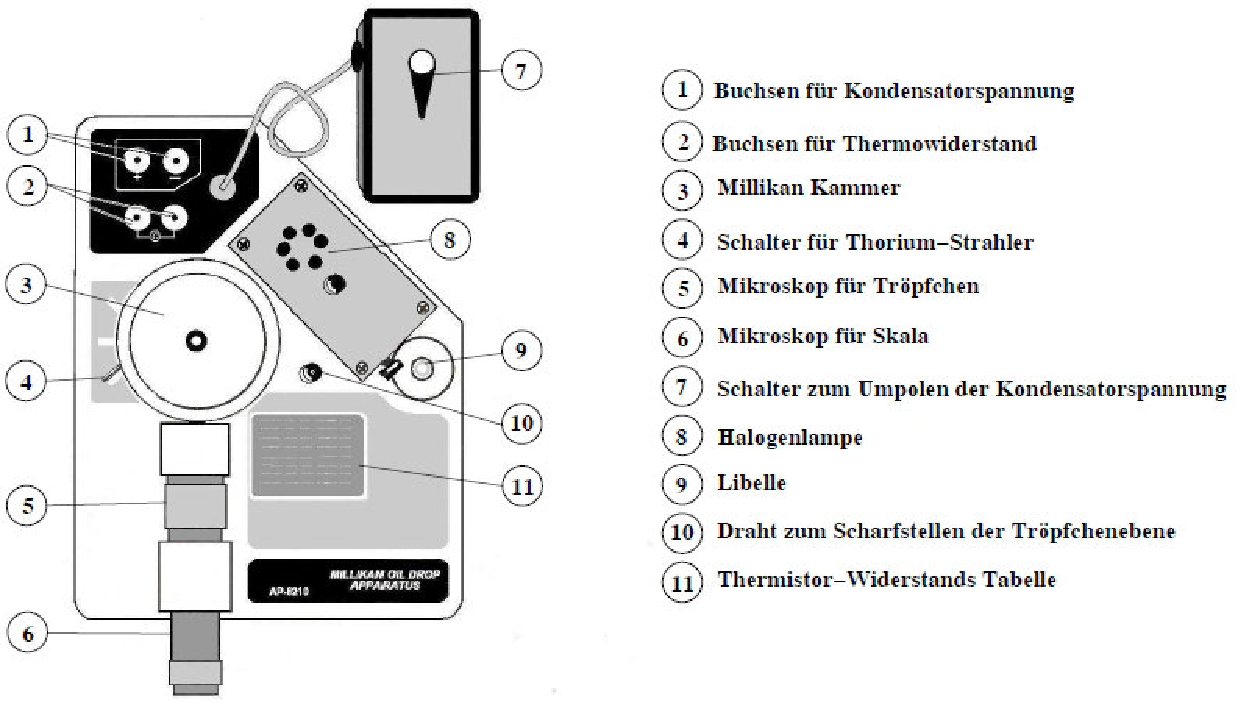
\includegraphics[scale=0.6]{Grafiken/Aufbau.pdf}
\caption{Der zu verwendende Aufbau für die Bestimmung der Elementarladung \cite{V503}.}
\label{Aufbau}
\end{figure}
Der hier Verwendete Plattenkondensator hat den Abstand $d=(7,6280\pm0,0051)$cm und die obere der beiden Platten besitzt ein Loch, durch dass das Öl in den zwischen Raum gelangt. Die Öltröpfchen werden durch eine Lampe Bestrahlt damit sie aufleuchten und sich gegen über des Hintergrundes abheben und sich durch das Mikroskop beobachten lassen. Zwar sind die meisten Tröpfchen elektrisch geladen, aber dennoch kann durch Hebel (4), die Abschirmung eines $\alpha$-Präparat entfernt werden, wodurch die Tröpfchen geladen werden, es ist darauf zu achten, dass während des Bestrahlens der Tröpfchen der Kondensator ausgeschaltet ist. Da sich der zwischen Raum durch die Lampe erhitzt, ist es notwendig den Widerstand des Thermoelementes zu messen. Der Kondensator kann durch Hebel (7) angeschaltet und die Polung eingestellt werden. Mithilfe der Justiernadel (10) wird das Mikroskop scharfgestellt.\\
Die Messung wird damit begonnen das die Öltröpfchen in den Kondensator gesprüht werden, wobei der Kondensator ausgeschaltet ist. Nun wird geladenes Tröpfchen beobachtet, ob es geladen ist kann überprüft werden in dem der Kondensator eingeschaltet wird. Für das Tröpfchen wird die Zeit für eine Strecke, ein mal mit der Geschwindigkeit $v_\text{ab}$ und für $v_\text{auf}$ gemessen, sowie einmal nach mehrerer Messungen $v_0$. Diese Messung wird für eine größere Anzahl an Tröpfchen wiederholt und für mehrere Spannungen, wobei die Spannung nicht über 500V  gehen sollte.

